\subsection{AI-Based Support Tools}

While tools such as ChatGPT were utilized transversally to support drafting, code refinement, and logical requirement analysis, the specific phase of User Interface Prototyping relied on models specialized in image generation.

\noindent
Specifically, Google AI Studio was employed to interact with the Gemini model. Thanks to its multimodal capabilities, it was possible to translate the textual descriptions of Use Cases into high-fidelity visual mockups. This approach allowed for a rapid visualization of the spatial organization of elements (layout).

\subsection{Example of Interaction: Mockup Generation}

 A significant example of this interaction is represented by the definition of the Homepage. Initially, a prompt was provided to the model aimed at establishing the general structure and color palette, inspired by leading market competitors.

\begin{PromptBox}
\quad Generate a mockup for the homepage of a mobile GPS navigation application. The interface must be in "Dark Mode", featuring a dark night-time street map background similar to Google Maps. At the bottom of the screen, include a navigation bar with four sections: "Home", "Published", "Recent Trip", and "Profile". Position two round floating buttons stacked vertically immediately above this bar in the bottom right corner: one for "Manual Mode" and the other for "Automated Mode".

\vspace{0.3cm}

\end{PromptBox}

\begin{GeminiBad}
\quad Here is a proposal for the Homepage design in night mode. The generated image presents: \begin{itemize} \item A dark-toned cartographic background (midnight blue and charcoal) with highlighted roads. \item A bottom navigation bar featuring the four requested sections. \item The two action buttons ("Manual" and "Automated") positioned at the bottom right for easy thumb access. \end{itemize}

\textbf{} \\
    \begin{center}
    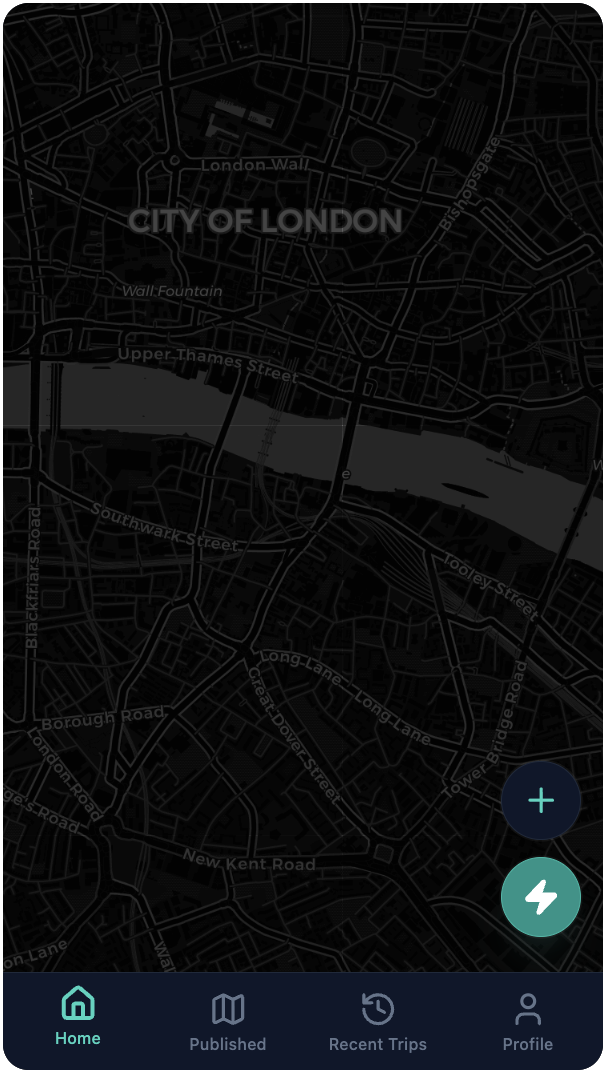
\includegraphics[height=6cm, keepaspectratio]{RASD/Images/WrongImage.png}
    \end{center}
    
\vspace{0.3cm}
\end{GeminiBad}

\noindent
Although the structure was correct, the first iteration lacked crucial elements for immediate usability, such as a clear indication of the user's position and the destination input field. A second refinement prompt was therefore necessary to integrate these details without altering the already approved visual style.

\vspace{0.3cm}
\begin{PromptBox}
\quad Based on the image just generated, modify only the top area and the center of the map. Add a floating search bar at the top of the screen specifically for entering a destination (with a placeholder like "Where to?"). Additionally, place a prominent cursor, such as a glowing blue arrow, in the center of the map to indicate the user's current position. Ensure that the rest of the existing interface, including the bottom navigation bar, remains unchanged.

\vspace{0.3cm}
\end{PromptBox}


\begin{GeminiGood}
\quad Updated the mockup by integrating the requested elements: \begin{itemize} \item \textbf{Search Bar:} Inserted at the top with rounded corners and a search icon, maintaining the transparency typical of modern UIs. \item \textbf{Position Cursor:} Added a blue indicator with a slight glow effect at the center of the map to ensure immediate contrast against the dark background. \end{itemize} The rest of the layout (navbar and mode buttons) remained unchanged.

\textbf{} \\
    \begin{center}
    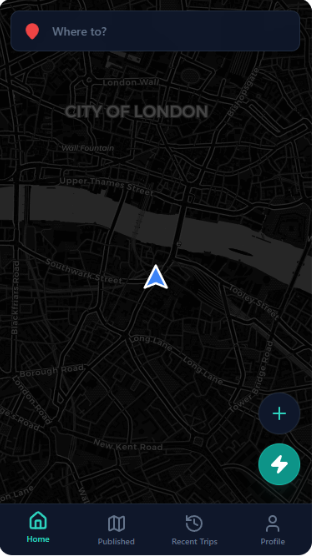
\includegraphics[height=6cm, keepaspectratio]{RASD/Images/TrueImage.png}
    \end{center}
    
\vspace{0.3cm}

\end{GeminiGood}

\vspace{0.5cm}



\noindent
This two-phase process allowed for the separation of the structural layout definition (navbar, map, buttons) from the functional details (search bar, cursor). The model demonstrated the ability to maintain stylistic consistency between generations, integrating the requested modifications naturally within the pre-existing visual context.

\newpage
\subsection{Example of Interaction: Rules Identification}

The following interaction describes a consultation aimed at defining the Standard Compliance section. We engaged the AI to clarify the complex requirements related to the handling of continuous geolocation history and the integration of external map services. Through two prompts, we progressed from identifying the applicable external regulations (GDPR, Terms of Service) to defining the internal technical solutions required to ensure compliance without compromising the platform’s functionality.

\vspace{0.5cm}

\begin{PromptBox}
\quad I am developing a mobile app for cyclists that features real-time navigation and trip tracking, relying on third-party map services. Considering I will be handling continuous geolocation data, what are the primary privacy regulations and map licensing constraints I need to strictly follow?

\vspace{0.3cm}

\end{PromptBox}

\begin{ChatGPTBad}
\quad Based on your description, the platform operates at the intersection of sensitive user data and proprietary services. Here are the mandatory constraints:
\begin{enumerate}
    \item Privacy and Sensitive Data: Since the system handles Personally Identifiable Information (PII) and continuous geolocation history, this constitutes a significant privacy risk as it reveals user habits and private locations. You must strictly comply with the General Data Protection Regulation (GDPR) and potentially the California Consumer Privacy Act (CCPA).
    \item Map Provider Terms of Service (ToS):The dependency on external providers (e.g., OpenStreetMap or Google Maps) mandates rigorous adherence to their ToS. You are required to:
    \begin{itemize}
        \item Dynamically display proper copyright attributions.
        \item Strictly enforce technical limitations on offline data caching to avoid licensing violations.
    \end{itemize}
\end{enumerate}
    
\vspace{0.3cm}
\end{ChatGPTBad}



\vspace{0.5cm}

\noindent
The analysis of the regulatory landscape revealed a critical tension: the application requires continuous data collection for functionality, yet strictly limits data retention for compliance. Recognizing that simple adherence to rules is insufficient, we directed the next query toward defining the architectural drivers necessary to resolve this conflict at the structural level.

\vspace{0.3cm}
\newpage
\begin{PromptBox}
\quad Based on these regulatory constraints, how should I design the software architecture to ensure compliance? Specifically, I need to understand how to embed "Privacy-by-Design" principles into the core system and how to technically enforce the caching limitations, while keeping the architecture flexible enough to adapt to future changes.

\vspace{0.3cm}
\end{PromptBox}


\begin{ChatGPTGood}
\quad To ensure compliance without compromising functionality, the system must be architected with specific drivers:
\begin{itemize} \item \textbf{Privacy-by-Design Core:} You must embed privacy-by-design principles directly into the software core, rather than treating compliance as an external add-on. This minimizes the risk of exposing user habits. \item \textbf{Adaptability and Flexibility:} The system must be architected with the flexibility to adapt to this dual set of regulatory and licensing constraints. Regulations and ToS change frequently; a modular design will allow you to update compliance logic without rewriting the entire application.\item \textbf{Technical Enforcement:} The architecture must include a logic layer that automatically manages data retention, ensuring you strictly enforce technical limitations on offline data caching as required by the map providers.\end{itemize} The rest of the layout (navbar and mode buttons) remained unchanged.
    
\vspace{0.3cm}

\end{ChatGPTGood}


\vspace{0.5cm}

\noindent \textbf{Verification} \\
We verified the information generated by the AI by checking official online sources. The details regarding privacy regulations and map service policies were confirmed to be accurate and consistent with real-world requirements. Therefore, the content is reliable and has been validated for use in this project.

\subsection{Conclusion}
The integration of AI-based tools has significantly improved efficiency in the preparation of complex technical documents. Nevertheless, despite their advantages, it remains essential to adopt a critical approach and carefully review the produced content to ensure accuracy, coherence, and completeness. Achieving high-quality results often requires multiple iterations and precise refinements, guiding the process step by step. AI tools have proven to be valuable support instruments, but they should be used with careful supervision throughout all phases of document development.